% !Mode:: "TeX:UTF-8"
%% 请使用 XeLaTeX 编译本文. 默认使用 Adobe 字体. 需自行安装.
%%文件名不能出现任何中文字,否则反向查询功能不能实现
%\documentclass{mytemplate}% 选项 forprint: 交付打印时添加, 避免彩色链接字迹打印偏淡. 即使用下一行:
\documentclass[forprint]{mytemplate}
\usepackage{abstract,float}
\usepackage{makecell}
\setmainfont{Times New Roman}

%%===参考文献===%%%%%%%%%%%%%%%%%%%%%%%%%%%%%%%%
\bibliographystyle{abbrv}        % 参考文献样式,  plain,unsrt,alpha,abbrv,chinesebst 等等
%%%%%%%%%%%%%%%%%%%%%%%%%%%%%%%%%%%%%%%%%%%
\graphicspath{{figures/}}        % 图片文件路径
%%%%%%%%%%%%%%%%%%%%%%%%%%%%%%%%%%%%%%%%%%%
\allowdisplaybreaks
%%%%%%%%%%%%%%%%%%%%%%%%%%%%%%%%%%%%%%%%%%%
%\setmainfont{Times New Roman}
\begin{document}
%%%%%%% 下面的内容, 据实填空.
\baselineskip=14pt  % 正文行距为 20 磅
\setlength{\columnsep}{20pt}

%----------------------------------------------------------------------------

\renewcommand{\thefootnote}{\fnsymbol{footnote}}
%\mytitle
%\simpletitle

%\coverpage

%\frontmatter
%\newpage
%\pagenumbering{arabic}%Roman  % 正文之前的页码用大写罗马字母(Roman)编号.也可选用arabic (阿拉伯数字)
%%-----------------------------------------------------------------------------
%\include{includefile/frontmatter}    % 加入摘要, 申明.
%==========================把目录加入到书签==============================%%%%%%
%\pdfbookmark[0]{目录}{toc}
\begin{flushleft}
{\zihao{-4} \heiti Midterm Report}
\end{flushleft}
\vspace{1cm}
\begin{center}
{\zihao{4}  \textbf{Marketing Campaign Candidate Analysis}}\\
{\zihao{5}Yiheng Xiao, Chen Zhong}
\end{center}
\vspace{0.5cm}
\begin{enabstract}
 Successful market Campaign boosts business by promoting products effectively. The important question here is how to choose the pool of potential customers to increase success rate. Our project is to propose a data mining approach to classify the best set of clients using contact records and clients' features. All Codes are in {\color{green}\texttt{"midterm.ipynb"}}.
\end{enabstract}
\vspace*{2em}
%%%%%%%%%%%%%%%%%%%%%%%%%%%%--------main matter-------%%%%%%%%%%%%%%%%%%%%%%%%%%%%%%%%%%%%

\setcounter{page}{1}
\setlength\parindent{0em}
\columnsep=20pt
\begin{multicols}{2}
\tableofcontents
\section{\color{blue} Project Introduction}
Marketing campaign is essential for any business in any industry to grow customers and expand business. A successful company requires not only good product but also a good way to advertise its product. One of the most traditional yet effective way of marketing campaign is through phone calls. These phone-call based marketing campaigns are done by making phone calls to a pool of potential customers to promote certain products. Unfortunately, in order to increase the rate of success many potential customers will be called more than once. While it takes a lot of time and effort to attract a new customer, very often people will feel uncomfortable about the repetitive phone calls and may even jeopardize the campaigning company’s reputation.

The important question here is how to choose the pool of potential customer to increase success rate? If we can increase
success rate of phone call marketing campaigns, less resource is required to attract each new customer and it is less likely
to have negative advertising effect.

Our approach to the problem is to analyze market campaign data, which includes information about the background of customers and try to determine the specific profile of customers who will be more likely to subscribe the product in campaign. More specifically, our project is to propose a data mining approach to select the best set of clients that are more likely to subscribe a product through tele-marketing calls.

\section{\color{blue}Initial Processing and Visualization}
\subsection{Raw Data}
We selected the Bank Marketing Data Set\footnote{http://archive.ics.uci.edu/ml/datasets/Bank+Marketing} from UCI Machine Learning repository. The data is taken from the direct marketing campaigns of a Portuguese banking institution. The marketing campaigns were based on phone calls. The data set consists of a list of 45211 samples with 20 features. We are interested in whether we can predict the "y" feature, which is the whether the particular sample subscribed to the product or not, using all other features given about that particular sample. Below is a list of sample important features {\color{red}Table \ref{t01}}.
\begin{table}[H]
  \centering
  \begin{tabular}{|l|l|l|}
     \hline
Client data & Description&Type \\ \hline
age & age of clients &numeric\\ \hline
 job & type of job&categorical\\ \hline
 marital & marital status&categorical\\ \hline
 education & level of education& categorical\\ \hline
 default & whether has credit in default& categorical\\ \hline
 housing & whether has housing loan& categorical\\ \hline
 loan  &whether has personal loan& categorical \\ \hline
   \end{tabular}
  \caption{Several Features}\label{t01}
\end{table}

\subsection{Initial Data Cleaning}
First thing we looked at was missing values. Besides the "poutcome" feature, most other features have similar amount of samples, to allow for initial steps, we filled the n/a values in "poutcome" with string "nonexistent" and proceeded to exclude all other n/a's, which result in a clean set of data with 30488 samples. We will try to preserve more data in the future.

Since we are dealing with many categorical and binary attributes, we used one hot encoding for categorical features (each category as a new feature and has binary value), and we transformed binary attributes to {0,1}. Which expands the data set to having 54 features. Reason for one-hot-encoding is that regression analysis requires numerical values, and each category as a feature allows our models to compare the affect of each category independently and makes it easier for us to eliminate some of the features.

\subsection{Visualization}
%![plot](https://github.com/Johnzhong1468/MarketingCampaign/blob/master/3d_age_dur_pd.PNG)<br>
\begin{figure}[H]
  \centering
  % Requires \usepackage{graphicx}
  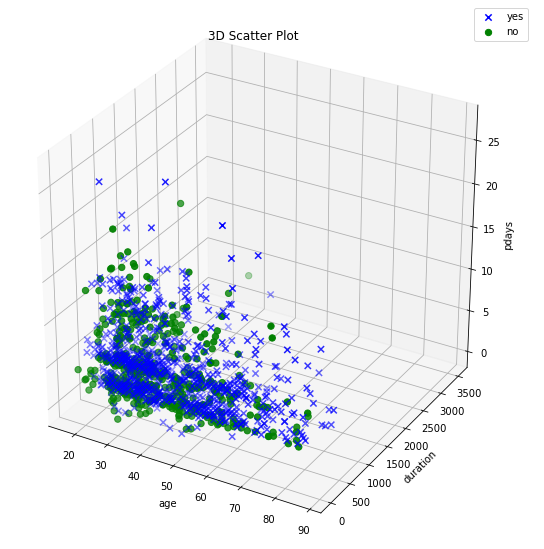
\includegraphics[width=9cm]{3d_age_dur_pd.PNG}\\
  \caption{Visualization 1}\label{g01}
\end{figure}

To First try to understand the data, we want to explore the relationship between some of the important features (see {\color{red}Graph \ref{g01}}), here we chose age, duration of previous contact(duration), and number of days past after previous contact(pday). We also restricted the data to people who have been contacted more than once. People who accepted the product are color coded with blue and those who didn't are green. We can see that there are a lot of people that actually accepted the product under the condition that they were contacted more than once. We can see that more samples have low duration and small pdays, and more samples are in the young age group than old age group. However for determining whether a sample accept the product, age does not seem to have a big effect graphically since "yes" samples have a similar profile as "no" sample. However duration and pday seem to have distinct affect, and we will explore that further in the future.
\begin{figure}[H]
  \centering
  % Requires \usepackage{graphicx}
  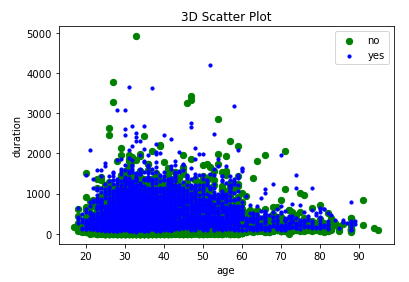
\includegraphics[width=7cm]{age_dur_scatter.PNG}\\
  \caption{Visualization 2}\label{g02}
\end{figure}

This plot shows the group of people who were only contacted once. We can see again that age has the same distribution profile among the "yes" and "no" group.
\begin{figure}[H]
  \centering
  % Requires \usepackage{graphicx}
  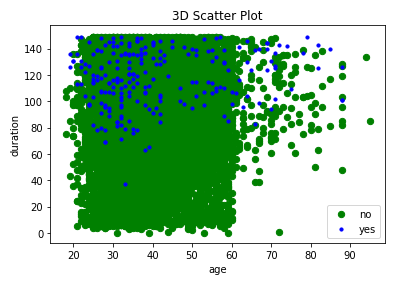
\includegraphics[width=7cm]{age_dur_scat_shrt.PNG}\\
  \caption{Visualization 3}\label{g03}
\end{figure}

%![plot](https://github.com/Johnzhong1468/MarketingCampaign/blob/master/age_dur_scat_shrt.PNG)<br>
We shrink duration to less than 150 and as expected people are likely to reject when the duration of the call is very short.

\section{\color{blue}Initial Model Selections}
\subsection{General Procedures}
The project focuses on a classification problem, so, we set a hypothesis set H including linear models with regularizer, Logistic regression models, Supporting Vectors Machine as well as Decision trees. To find the model with satisfying explanatory ability, the model selection obeys the following procedures:

\begin{enumerate}
  \item ~~Fit models in training set, remove non-significant features.
  \item ~~Select the optimal hyper-parameters by cross validation.
  \item ~~Compare the Prediction Accuracy computed on traning set and testing set.
  \item ~~Analyze results of different models.
\end{enumerate}
\subsection{Lasso Model}
Lasso regression performs covariate selection as well as improves prediction error by shrinking large regression coefficients in order to reduce overfitting. However, it may not effective in solving classification problems; the accuracy of Lasso is merely 4.22\%, which fails to meet our expectation.
\begin{equation}\label{eq01}
  \min \sum_{i=1}^n(y_i-w^Tx_i)^2+\lambda\sum_{i=1}^n|w_i|
\end{equation}
\subsection{Logistic Model}
The binary logistic model is designed to estimate a binary response based on predictor features. By cross validation, we calculate the penalty parameter ($\lambda$) that minimizes the percent of misclassifications. Some features are of non-significance. Thus, we prefer to remove them form the model, such as 'euribor3m' and 'nr.employed'. After dimension reduction, the accuracy shifts from 0.8875 to 0.8880, namaly, discarding ineffective features does not impair the model. The test accuracy is 0.8916.
\begin{equation}\label{eq02}
  \sum_{i=1}^n\log(1+e^{-y_iw_ix_i})+\lambda\sum_{i=1}^n|w_i|
\end{equation}
\subsection{Support Vector Machine}
Another typical classification we considered is SVM. Using one-hot-encoding, we get a sparse matrix of features, and SVM  has proven to offer significant advantages in dealing with large sparse datasets. We optimize the penalty parameter as C=0.6. The training and testing accuracy is 0.8848 and 0.8879, respectively. Thus, SVM provides highly explanatory classifications.

\subsection{Random Forests (Decision Trees)}
The way random forest works is that it randomly samples from the training set while maintaining the underling distribution. Then, it creates a series of decisions trees where each tree comprise a fixed amount of variables. Each decision tree is generated maximizing information efficiency (greatest reduction in entropy). In prediction, a majority score(vote) is taken from each group of decision trees to classify each client.

For our models, we initially fit a single decision tree (see {\color{red}Graph \ref{g04}}) as a pilot trial. We allowed the tree to grow to a max depth of 5, and find that the training and testing accuracy are around 0.88, which does not show the prominence of tree models. This attempt spurs us to increase the max depth and pursue a more flexible model, the random forests.

\begin{figure*}[!htp]
  \centering
  % Requires \usepackage{graphicx}
  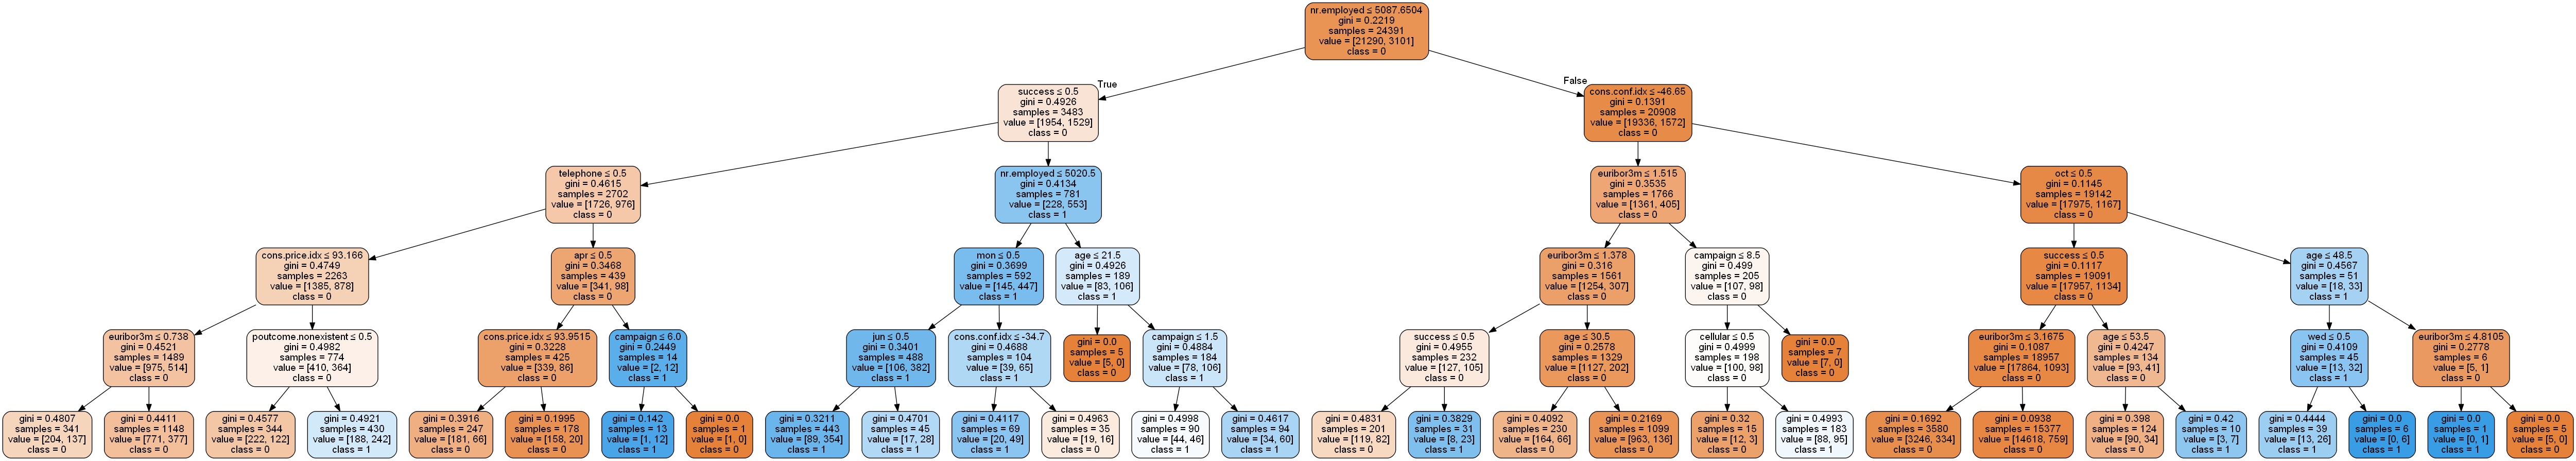
\includegraphics[width=4.5cm]{tree.png}\\
  \caption{Single Decision Tree}\label{g04}
\end{figure*}

%![plot](https://github.com/Johnzhong1468/MarketingCampaign/blob/master/tree.png)<br>

For our random forest model, we used 10 trees (especially less than the number of features) in our forest. We set trees to grow to a maximum depth of 20 and assigned trees to randomly pick the square root of the total number of features to split upon. We will prune the trees later in the second half of the semester, to boost the prediction.

Random forest is not prone to overfitting since the majority vote prevents weighing heavily on single classification. Moreover, it prevents underfitting since trees are randomly assigned to a subset of features.

\section{\color{blue}Summary of Preliminary Results}
Going through the general procedure mentioned in previous part, we fit each model and estimate their performance. The critical part of results are listed below. To test the effectiveness, we calculated accuracy as the percentage of correctly classified customers. We found that logistic regression, the SVM and random forest are able to classify with an accuracy of 89.16\%, 88.80\% and 87.85\%, respectively (See {\color{red}Table \ref{T02}}).

An indication that the great spread between the accuracy of the test data and training data for random forest is that the model requires further improvement, such as bagging. We will move forward in the second half of the semester.

\begin{table}[H]%[!htp]
  \centering
  \begin{tabular}{|l|c|c|l|}
     \hline
 Model   & \makecell[tl]{Training \\Accuracy} & \makecell[tl]{Testing\\ Accuracy} &Note\\ \hline
Lasso & 0.0422 &N.A. & Discarded\\ \hline
 Logistic & 0.8880 & 0.8916& generalization\\ \hline
 SVM & 0.8848 & 0.8880&generalization\\ \hline
\makecell[tl]{Decision Tree\\(depth=5)} &0.8923 &0.8896&-\\ \hline
\makecell[tl]{Decision Tree\\(depth=20)} &0.9702 &0.8432&-\\ \hline
Random Forest& 0.9572 & 0.8785&generalization\\ \hline
   \end{tabular}
  \caption{Preliminary Results}\label{T02}
\end{table}


\section{\color{blue}Future Steps}
\begin{description}
  \item[1.]~~ Preserve more data during the cleaning process. For example, treat n/a's as a new category and fill the gap.
  \item[2.] ~~Eliminate some redundant features using lasso or other models.
  \item[3.] ~~Explore the specific effect of particular features
  \item[4.] ~~A more robust comparison of models, using cross validation, and maybe mix up different models for better result
  \item[5.]~~ Further examine our models' level of generalization and overfitting, we don't yet have a good metric to determine
\end{description}
 \end{multicols}
\end{document}


